\documentclass[border={0pt 0pt 0pt 5pt}]{standalone}
\usepackage{pgfplots}
\usetikzlibrary{pgfplots.groupplots}
\usetikzlibrary{arrows.meta}
\usepackage{siunitx}
\pagecolor{white}
\begin{document}
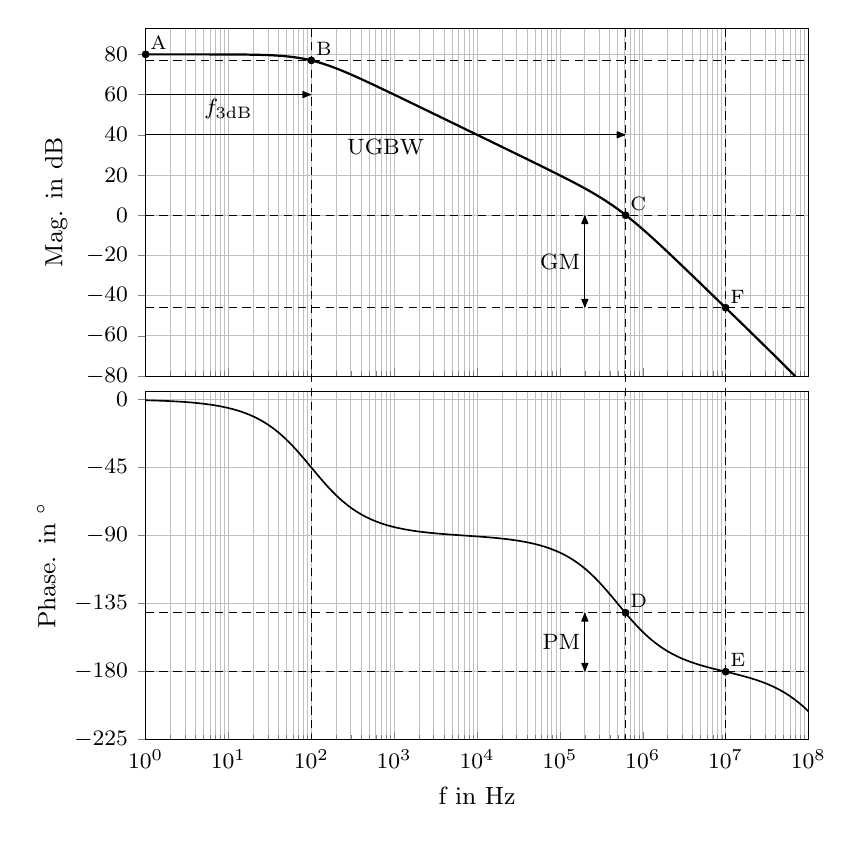
\begin{tikzpicture}
\begin{groupplot}[
  group style={ group name=my plots
              , group size=1 by 2
              , xlabels at=edge bottom
              , xticklabels at=edge bottom
              , vertical sep=2mm
              }
    , footnotesize
    , xmode=log
    , width=10cm
    , height=6cm
    , xlabel=f in \si{\hertz}
    , xmin=1
    , xmax=1e8
    , ymin=0
    , ymax=29
    , tickpos=left
    , ytick align=outside
    , grid=both
    , grid style={line width=0.3pt}
    , domain=1:1e8
    , samples=200
    ]

\nextgroupplot[ ymin=-80
              , ymax=93
              , ylabel= Mag. in \si{\decibel}
              ]

  \addplot[thick] 
    ({\x},{80-10*log10(1+(\x/1e2)^2)
             -10*log10(1+(\x/5e5)^2)
             -10*log10(1+(\x/2e8)^2)});

  \coordinate (f3dbtop) at (axis cs:1e2,\pgfkeysvalueof{/pgfplots/ymax});
  \draw [densely dashed] (axis cs:1e0,0) -- (axis cs:1e8,0);
  \draw [densely dashed] (axis cs:1e0,77) -- (axis cs:1e8,77);
  \draw [densely dashed] (axis cs:1e0,-46) -- (axis cs:1e8,-46);

  \coordinate (ugbwtop) at (axis cs:6.2e5,\pgfkeysvalueof{/pgfplots/ymax});

  \coordinate (coftop) at (axis cs:1e7,\pgfkeysvalueof{/pgfplots/ymax});

  \addplot[only marks,mark=*,mark options = {scale=0.6}] coordinates{
    (1,  80)  
  };

  \node[anchor=south west,font=\scriptsize, inner sep=1.5pt] 
    () at (axis cs: 1,80) {A};  

  \addplot[only marks,mark=*,mark options = {scale=0.6}] coordinates{
    (1e2,  77)  
  };

  \node[anchor=south west,font=\scriptsize, inner sep=1.5pt]  
    () at (axis cs: 1e2,77) {B};  

  \addplot[only marks,mark=*,mark options = {scale=0.6}] coordinates{
    (6.2e5,  0)  
  };

  \node[anchor=south west,font=\scriptsize, inner sep=1.5pt] 
    () at (axis cs: 6.2e5,  0) {C};  

  \addplot[only marks,mark=*,mark options = {scale=0.6}] coordinates{
    (1e7, -46)  
  };

  \node[anchor=south west,font=\scriptsize, inner sep=1.5pt] 
    () at (axis cs: 1e7,  -46) {F};  

  \draw[ {Latex[round,scale=0.8]}-{Latex[round,scale=0.8]}]
    (axis cs: 2e5,-46) -- (axis cs: 2e5,0) 
    node[midway, left, font=\footnotesize, inner sep=1.5pt] () {GM};

  \draw[-{Latex[round,scale=0.8]}]
    (axis cs: 1,60) -- (axis cs: 1e2,60) 
    node[midway, below, font=\footnotesize, inner sep=1.5pt] () {$f_{\mathrm{3dB}}$};

  \draw[-{Latex[round,scale=0.8]}]
    (axis cs: 1,40) -- (axis cs: 6.2e5,40) 
    node[midway, below, font=\footnotesize, inner sep=1.5pt] () {UGBW};

\nextgroupplot[ ymin=-225
              , ymax=5
              , ylabel= Phase. in \si{\degree}
              , ytick={0,-45,-90,-135,-180,-225}
              ]

  \addplot[semithick]({\x},{-atan(x/1e2)-atan(x/5e5)-atan(x/2e8)}); 

  \coordinate (f3dbbot) at (axis cs:1e2,\pgfkeysvalueof{/pgfplots/ymin});

  \draw [densely dashed] (axis cs:1e0,-180) -- (axis cs:1e8,-180);

  \coordinate (ugbwbot) at (axis cs:6.2e5,\pgfkeysvalueof{/pgfplots/ymin});
  \coordinate (cofbot) at (axis cs:1e7,\pgfkeysvalueof{/pgfplots/ymin});

  \draw [densely dashed] (axis cs:1e0,-141) -- (axis cs:1e8,-141);

  \addplot[only marks,mark=*,mark options = {scale=0.6}] coordinates{
    (6.2e5,-141)  
  };

  \addplot[only marks,mark=*,mark options = {scale=0.6}] coordinates{
    (1e7,-180)  
  };

  \node[anchor=south west,font=\scriptsize, inner sep=1.5pt] 
    () at (axis cs: 6.2e5,  -141) {D};  

  \node[anchor=south west,font=\scriptsize, inner sep=1.5pt] 
    () at (axis cs: 1e7,  -180) {E};  

  \draw[ {Latex[round,scale=0.8]}-{Latex[round,scale=0.8]}]
    (axis cs: 2e5,-180) -- (axis cs: 2e5,-141) 
    node[midway, left, font=\footnotesize, inner sep=1.5pt] () {PM};
\end{groupplot}

\draw [densely dashed] (f3dbtop) -- (f3dbbot);
\draw [densely dashed] (ugbwtop) -- (ugbwbot);
\draw [densely dashed] (coftop) -- (cofbot);

\end{tikzpicture}
\end{document}